\chapter{Elastic linear plate}

\modinfo{Directory}{ElasticPlateLinear}
\modinfo{Solvers}{\Idx{SmitcSolver}}
\modinfo{Tools}{\Idx{ElmerGrid}, editor}
\modinfo{Dimensions}{2D}

\subsection*{Case definition}

This tutorial demonstrates how to use the Smitc solver to solve
small deflections of plates.
The Smitc solver is for elastic linear plates and
uses the theory of Reissner and Mindlin.

The case under investigation is a L-shaped steel plate under pressure.
The plate is shown in figure~\ref{fig:simplePlate}
The longer sides have the length of $2\,m$ and the shorter $1\,m$. 
So the area of the plate is $3\,m^2$. The plate has a thickness of
$1\,cm$. We assume that on the plate
there is about $15300\,kg$ of sand. The sand is uniformly distributed
on the plate and the sand stays uniformly distributed even if the 
plate undergoes small deflection. The sand exerts to the plate
a pressure of $50000\,Pa$. The plate is clamped from all sides
meaning that both deflection and rotation are zero on all edges.
%
\begin{figure}[tbhp]
\begin{center}
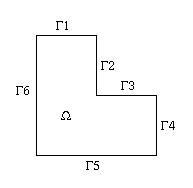
\includegraphics[width=0.4\textwidth]{simplePlate}
\end{center}
\caption{The geometry of plate and the numbering of edges.}
\label{fig:simplePlate}
\end{figure}

\subsection*{Solution Procedure}

The first thing to do is create a mesh with ElmerGrid.
The definition of mesh is in the file \texttt{simple\_plate.grd}.
The mesh is about uniform and consist of 1000 linear square elements.
The mesh is created with command
\ttbegin
ElmerGrid 1 2 simple_plate
\ttend
One thousand element should easily do the trick in this case
but if more elements is needed you can edit the file 
\texttt{simple\_plate.grd}.
More specifically the line
\ttbegin
Surface Elements = 1000
\ttend

The solver input file \texttt{simple\_plate.sif} starts with turning on 
the warnings and the definition of the proper mesh directory. 
%
\ttbegin
check keywords warn

Header
  Mesh DB "." "simple_plate"
End
\ttend
The simulation uses 2D cartesian geometry. The simulation is not
time dependent i.e. Steady State. 
There is no coupled solvers so only one iteration is needed. 
The output interval is one meaning all intervals (now there is only one
interval). Numerical results are written to file \texttt{simple\_plate.result}
and ElmerPost file is \texttt{simple\_plate.vtu}.
\ttbegin
Simulation
  Coordinate System = Cartesian 2D
  Simulation Type = Steady State
  Steady State Max Iterations = 1
  Output Intervals = 1
  Output File = "simple_plate.result"
  Post File = "simple_plate.vtu"
End
\ttend
There is just one body, the plate, and it uses Equation and  Body Force 1 and
is of Material 1.
\ttbegin
Body 1
  Equation = 1
  Body Force = 1
  Material = 1
End
\ttend
The equation block is now more than easy. 
It only states that we use Solver 1 to solve the equation.
\ttbegin
Equation 1
  Active Solvers(1) = 1
End
\ttend
In Body Force block we give the equations right hand side. 
It is the sands pressure and it is the same constant in every point.
\ttbegin
Body Force 1
  Pressure = 5.0e4
End
\ttend
In Material block we define the plates properties i.e. Poisson ratio,
Young's modulus and density. We also give the plates thickness and
possible pretension. Now there is no pretension.
\ttbegin
Material 1   
  Poisson ratio = 0.3
  Youngs modulus = 209e9
  Density = 7800.0

  Thickness = 1.0e-2
  Tension = 0.0
End
\ttend
Next the Solver block.
\begin{itemize}
\item First we define that we use SmitcSolver  
and give the name of the subroutine file \texttt{Smitc} and
subroutine name \texttt{SmitcSolver}. 
\item We name the variable Deflection and state that it has 3 degrees of freedom. 
First degree is the deflection and the remaining two are actually 
the components of rotation vector. 
\item We don't need eigen analysis nor is there any holes in the plate. 
\item We solve the matrix equation iteratively with stabilized biconjugate 
gradient method. We precondition the iteration with incomplete 
LU-factorization. 
\item Tolerance for the matrix system is $1\cdot10^{-8}$
and the tolerance should be achieved in less than 300 iteration.
\end{itemize}
\ttbegin
Solver 1
  Equation = "SmitcSolver"
  Procedure = "Smitc" "SmitcSolver"

  Variable = Deflection
  Variable DOFs = 3

  Eigen Analysis = False
  Hole Correction = False

  Linear System Solver = Iterative
  Linear System Iterative Method = BiCGStab
  Linear System Preconditioning = ILU2
  Linear System Convergence Tolerance = 1.0e-8
  Linear System Max Iterations = 300
End
\ttend
Finally we give the boundary conditions. The plate has 6 edges and
the edge numbering is in figure~\ref{fig:simplePlate}. All the edges are
clamped i.e. no deflection (Deflection 1) and  no rotation (Deflection 2 and 3).
\ttbegin
Boundary Condition 1
  Target Boundaries(6) = 1 2 3 4 5 6
  Deflection 1 = 0.0
  Deflection 2 = 0.0
  Deflection 3 = 0.0
End
\ttend

\subsection*{Results}

The problem is solved in few seconds and the results are viewed historically with ElmerPost. Currently you would use Paraview or something that can read the
VTU files. Here the results are still shown as originally done in ElmerPost.

Note that the 1st component of Deflection is the displacement to normal
direction whereas the 2nd and 3rd components are the x- and y-components of
rotation vector.

Result is shown in figure~\ref{fig:simplePlateDeflection}.
%
\begin{figure}[tbhp]
\begin{center}
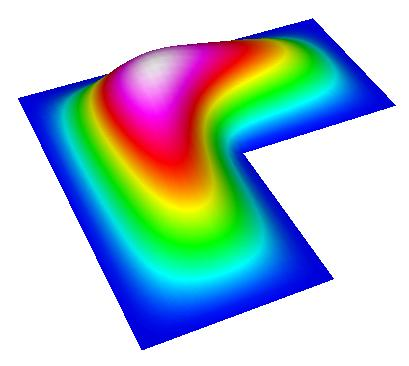
\includegraphics[width=0.48\textwidth]{simplePlateDeflection}
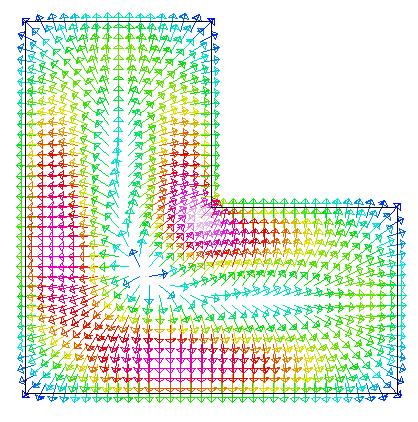
\includegraphics[width=0.48\textwidth]{simplePlateRotation}
\end{center}
\caption{The deflection of the plate and the corresponding rotation.}
\label{fig:simplePlateDeflection}
\end{figure}
%
%\begin{figure}[tbhp]
%\begin{center}
%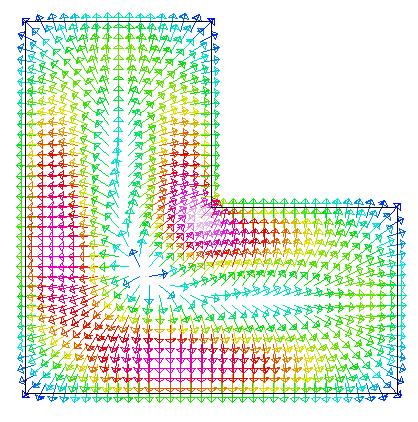
\includegraphics[width=0.5\textwidth]{simplePlateRotation}
%\end{center}
%\caption{The rotation of the plate.}
%\label{fig:simplePlateRotation}
%\end{figure}

